\documentclass[11pt]{scrreprt}

% TODO
% napisati nešto o igranju u parovima, kako to može narasti i do igranja među školama
% priložiti anketu i izbrisati "Budući da je anketa prevelika...""
% dodati grafove o odgovorima profesora o tome koliko im je spretno i zanimljivo koristiti aplikaciju

\usepackage[croatian]{babel}
\usepackage[utf8]{inputenc}
\usepackage[T1]{fontenc}
\usepackage{hyperref}
\usepackage{graphicx}
\usepackage{tikz}
\usepackage{pgfplots}
\usepackage{float}
\usepackage[nottoc,numbib]{tocbibind}
\usepackage{color}
\usepackage{multicol}
\usepackage[export]{adjustbox}
\usepackage{url}
\usepackage[stable]{footmisc}
\usepackage{chngcntr}
\usepackage{wrapfig}
\usepackage[
  left = \frqq,%
  right = \flqq,%
  leftsub = \frqq,%
  rightsub = \flqq,%
]{dirtytalk}

\setlength{\parskip}{\bigskipamount}
\setlength{\parindent}{0pt}
\linespread{1.5}
\graphicspath{ {./images/} }
\counterwithout{footnote}{chapter}
\setlength{\abovecaptionskip}{0pt}

\begin{document}

\begin{titlepage}
\pagenumbering{roman}

\begin{center}

  Sveučilište u Zagrebu\\
  Filozofski fakultet\\
  Odsjek za informacijske i komunikacijske znanosti\\
  Akademska godina 2013/14.

  \vspace*{150pt}

  { \huge Kvizovi kao alternativni način učenja }

  \vfill

  { \large Studenti: Janko Marohnić i Matija Marohnić\\
  Mentorica: doc. dr. sc. Kristina Kocijan }

  \vspace*{40pt}

  Zagreb, 2014.

\end{center}

\end{titlepage}

\pagebreak

\vspace*{240pt}

Ovaj je rad izrađen na Odsjeku za informacijske i komunikacijske znanosti
Filozofskoga fakulteta u Zagrebu pod vodstvom doc. dr. sc. Kristine Kocijan i
predan je na natječaj za dodjelu Rektorove nagrade u akademskoj godini
2013/2014.

\pagebreak

\tableofcontents

\chapter{Uvod}

\pagenumbering{arabic}

Zbog stalne izloženosti brzo mijenjajućim tehnologijama, umreženosti na
različitim razinama i korištenjem različitih uređaja, učenici imaju sve više
poteškoća s tradicionalnim oblicima učenja, a njihova koncentracija i motivacija
pada. Učenici nerijetko ne vide smisao u savladavanju velike količine gradiva
kada većinu informacija jednostavno mogu pronaci putem web tražilica. Jedan od
razloga pomanjkanja motivacije je i sporo mijenjanje obrazovnog sustava, koji
uglavnom ne slijedi promijene koje se zbivaju s novim generacijama učenika.\cite{perisic13}

Postoje razni kreativni načini da se upotrijebi informacijska tehnologija u
nastavi:

\begin{itemize}
  \item prezentacije (koristeći aplikacije kao što je npr. \emph{Microsoft
    PowerPoint})
  \item digitalne ilustracije (npr. u biologiji, povijesti i sl.)
  \item digitalne simulacije (npr. u fizici i kemiji)
  \item video zapisi (npr. za nastavu povijesti) itd.
\end{itemize}

Međutim, to je obično prilično jednostrano, u smislu da samo profesori koriste
tehnologiju dok ih učenici gledaju. Ljudi bolje uče i više se zanimaju za
gradivo kroz interakciju. Smatramo da se trebaju razvijati puno interaktivnije i
zabavnije metode podučavanja.

Profesori koji su spremni koristiti interaktivne alate za podučavanje nemaju velik
izbor, jer je većina dobrih alata na engleskome jeziku, što predstavlja problem
mlađim generacijama učenika koja još ne znaju dobro engleski ili profesorima
koji ga nikad nisu učili u školi (jer su umjesto engleskog imali njemački,
francuski ili pak ruski). Potreban je jednostavan alat koji je namijenjen
hrvatskoj populaciji.

U potrazi za alternativnijim pristupima podučavanja kojeg učenici ne nalaze u
hrvatskim školama 21. stoljeća, odlučili smo razviti jedan takav sustav kako bi
smo, uz pomoć tehnologije, učenike pokušali zainteresirati za gradivo koje
obrađuju te ga tako barem djelomično približili učeniku 21. stoljeća kakvi
sjede npr. u američkim i japanskim školama. Iako se sustav može proširiti i na
druge predmete, mi smo se u prvoj testnoj fazi orijentirali na nastavnike
hrvatskoga jezika s posebnim naglaskom na sate lektire. Program smo testirali u
periodu od skoro dvije godine te ga za to vrijeme neprestano usavršavali i
nadopunjavali novim mogućnostima. U ostatku rada izložit ćemo naše osnovne
hipoteze kojima smo se vodili u ovom projektu. Potom ćemo detaljno opisati
program koji smo napravili iz perspektive nastavnika, studenta, ali i
programera. Na kraju ćemo prikazati i rezultate koje smo dobili uz pomoć anketa
i praćenja korisnika za vrijeme njihova korištenja aplikacijom.

\section*{Postojeće aplikacije}

Jedan od najjednostavnijih načina ispitivanja znanja je rješavanje kvizova,
stoga smo pretraživali hrvatske i strane aplikacije koje se bave tom temom.
Ovdje ćemo navesti i ukratko opisati neke od njih.

\begin{description}

  \item[Kvizovi.net] je srpska aplikacija za kvizove iz mnogih područja kao što
    su glazba, zemljopis, sport, povijest, filmovi i serije. Osim kvizova, u
    aplikaciji se nalaze i igre te vicevi, ali kompletan sadržaj ove aplikacije
    je vrlo oskudan zbog toga što je mogu izmjenjivati jedino autori
    aplikacije, nema baze korisnika koji mogu stvarati i rješavati kvizove pa
    prema tome skupljati bodove i sl.\cite{kvizovinet}

  \item[Kvizoteka] je, kao i \emph{Kvizovi.net}, kolekcija besplatnih kvizova iz
    svih područja kao što su filmovi, povijest, opće znanje, sport, glazba itd.
    Osim kvizova, nudi i popularne igrice kao što su Pacman, Tetris, Super Mario
    itd. Za razliku od \emph{Kvizovi.net}, \emph{Kvizoteka} ima bazu korisnika i
    neke statističke informacije o kvizovima.\cite{kvizoteka}

  \item[Učionica] je iOS\footnote{Mobilni operacijski sustav koji razvija
    Apple.} aplikacija namijenjena djeci predškolske dobi, pomaže im svladati
    osnovne pojmove kao što su abeceda, životinje, brojevi, oblici, boje i
    vrijeme. Ipak, rješenje koje mi tražimo odnosi se na djecu osnovnoškolske i
    srednjoškolske dobi. Nedostatak joj je to što je dostupna samo za iOS, nije
    je još moguće koristiti na ostalim mobilnim operacijskim sustavima niti na
    desktop ili laptop računalima. Također, slabijega je dizajna, ima loše
    ocjene korisnika i naplaćuje se 3 USD.\cite{ucionica}

  \item[QuizUp] je vrlo kvalitetna i popularna aplikacija za kvizove na
    engleskom jeziku. Od navedenih, ova aplikacija je najviše opsežna i ažurna i
    ima najviše mogućnosti. Osim rješavanja kvizova, korisnici \emph{QuizUp}-a
    ih mogu i stvarati ako žele. Za razliku od ostalih navedenih aplikacija,
    \emph{QuizUp} ima puno izraženiji socijalni aspekt i upotrebu
    gejmifikacije\footnote{Korištenje elemenata iz igara u drugim kontekstima.},
    koja potiče rješavanje kvizova, tako što korisnici dobivaju bodove i prema
    njima im se dodjeljuju određeni statusi. Nedostatak je ove aplikacije što
    je dostupna na engleskome jeziku i samo na mobilnim uređajima, nije je
    moguće igrati na desktop i laptop računalima.\cite{quizup}

\end{description}

S obzirom na to da nismo našli nijedno prihvatljivo rješenje za hrvatsku
aplikaciju za kvizove, počeli smo razvijati svoju i nazvali smo ju
\emph{Kvizovi} (\url{http://kvizovi.org}). To je aplikacija za rješavanje
kvizova koja je prilagođena za osnovne i srednje škole u Hrvatskoj. Prepoznaje
2 osnovna tipa korisnika -- \textbf{učenike} i \textbf{profesore}. U ovom smo
istraživanju testirali \emph{Kvizove} na nekoliko osnovnih i srednjih škola.

\chapter{Hipoteza}

Cilj ovog istraživanja bio je saznati:

\begin{enumerate}
  \item Pomaže li ovakav način učenja učenicima da bolje savladaju gradivo?
  \item Čini li aplikacija profesorima podučavanje zanimljivijim?
\end{enumerate}

Naša prva pretpostavka je bila da će oni učenici koji su učili rješavajući
kvizove pomoću naše aplikacije biti više zainteresirani za gradivo te da će ga i
bolje usvojiti u odnosu na učenike koji su učili klasičnim pristupom, tj.
slušajući predavanja. Učenici rješavanje kvizova mogu gledati kao na neku vrstu
igre, što može pozitivno utjecati na usvajanje znanja. Interes za gradivo može
potaknuti i mogućnost igranja u paru, odnosno natjecanja s drugim učenicima.

Druga pretpostavka bila je da će profesorima ispitivanje učenika pomoću
aplikacije za kvizove biti jednostavnije i informativnije nego ispitivanje na
tradicionalne načine kao što su sastavljanje testova i usmeno ispitivanje. Može
biti jednostavnije zato što kviz trebaju sastaviti jednom i mogu koristiti alat
koji je specijaliziran za kvizove, ne moraju ih tiskati i ne moraju ih ručno
ispravljati kasnije, to se događa automatski prema točnim odgovorima koje su
profesori unijeli. A može biti informativnije zato što profesori dobivaju puno
podataka o tome kako njihovi učenici rješavaju kvizove, koliko im je trebalo za
svako pitanje, kada su točno bili gotovi, s kime su igrali itd.

Možemo uzeti u obzir da prema VAK principu dijelimo ljude prema tri različita
tipa -- vizualni, auditivni i kinestetički.\cite{clark11} Smatramo da
ćedijelimo ljude prema tri različita tipa naša aplikacija najviše pomoći onima
koji najbolje uče preko vizualnih i kinestetičkih podražaja.

\chapter{Aplikacija}

Istraživanje smo proveli tako što smo izradili aplikaciju za kvizove i dali
određenom uzorku osnovnih i srednjih škola na testiranje (vidi poglavlje
\ref{chap:results}). Izvorni kôd aplikacije javno je dostupan na web aplikaciji
GitHub (\url{https://github.com/twin/kvizovi}), te ga zbog toga nećemo posebno
prilagati. Kôd je pod MIT licencom, koja omogućava svime da vide kako
aplikacija funkcionira, promatrati kako se razvijala kroz vrijeme, doprinijeti
aplikaciji na bilo koji način, pa čak i napraviti svoju kopiju aplikacije i
razvijati je na svoj način.\cite{mit}

Kreirali smo i blog na kojemu obavještavamo korisnike o ažuriranju aplikacije.
Uz blog smo kreirali i vodič kroz aplikaciju koji je dostupan u bilo kojem
trenutku svim korisnicima (nastavnicima i učenicima) kako bismo im olakšali
korištenje aplikacije. Također, u slučaju bilo kakvog problema ili poteškoća,
korisnici su nas uvijek mogli kontaktirati na e-adresama koje se nalaze unutar
kontakt sekcije u glavnoj navigaciji (prema rezultatim ankete, korisnici su
bili zadovoljni sa snalaženjem u aplikaciji i obaviještenošću o promjenama --
njih 60\% je reklo da se dobro snalaze, a njih 80\% je reklo da su zadovoljni
obaviještenošću promjenama).\cite{krug05}

Korisnici također mogu naknadno izmjenjivati svoje podatke u korisničkom
računu.

\pagebreak

Korisnik započinje korištenje aplikacije tako da odabere svoju ulogu u školi
(sliku \ref{fig:home}). Ovisno o odabranoj ulozi, aplikacija pruža drugačiju
funkcionalnost.

\begin{figure}[H]
  
\includegraphics[width=\textwidth, clip=true, trim=0 7cm 0 0, fbox]{home}
  \caption{Početna stranica}
  \label{fig:home}
\end{figure}

\section{Izrada aplikacije}

\emph{Kvizovi} su web aplikacija, dakle koristi se pomoću web preglednika. Sa
strane klijenta (web preglednika) koristimo tehnologije kao što su HTML, CSS i
JavaScript, a sa strane poslužitelja koristimo programski jezik Ruby i
PostgreSQL relacijsku bazu. U narednim poglavljima ukratko opisujemo svaku od
tehnologija.

\subsection{Tehnologije na strani klijenta}

Ove tehnologije izvršavaju web preglednici te su one jedinstvene, odnosno za
njih ne postoje alternative. Specifikacije ovih tehnologija razvija međunarodna
organizacija W3C (World Wide Web Consortium).

\subsubsection{HTML}

HTML je jezik kojim se označava sadržaj i struktura web stranica, te sam po sebi
ne propisuje izgled, već web preglednik ima unaprijed definirana CSS pravila za
izgled svakog HTML elementa u slučaju da web dizajner nije definirao
svoja.\cite{htmlncss}

Za našu aplikaciju koristili smo najnoviju verziju HTML-a -- HTML5. Koristili
smo je zbog novih funkcionalnosti koje pruža, kao što je povezivanje računala
što omogućuje nove značajke u aplikaciji, na primjer grupno rješavanje kvizova.
\cite{diveintohtml5}

\subsubsection{CSS}

CSS je stilski jezik koji se koristi za opis prezentacije HTML dokumenata. Svaka
vrsta web preglednika ima drugačije implementiranu specifikaciju CSS-a zbog čega
ga ponekad interpretira malo drugačije od ostalih preglednika. Zato je složeno
napisati CSS na način da isto izgleda u svim web preglednicima.\cite{htmlncss}

Za našu aplikaciju koristili smo najnoviju verziju CSS-a -- CSS3. Velik dio CSS3
specifikacije implementiran je u modernim web preglednicima, a u starijim se web
preglednicima izgled aplikacije mjestimično elegantno degradira, što ne utječe
negativno na njezinu funkcionalnost. Za pregledavanje podržanosti pojedinih CSS3
stilova u web preglednicima koristimo bazu podataka \url{http://caniuse.com}.

\subsubsection{JavaScript}

JavaScript je skriptni programski jezik koji se koristi za dinamičku
manipulaciju HTML-a i komunikaciju s poslužiteljem. Dok su drugi jezici obično
sintaktički funkcijski ili objektni, JavaScript se temelji na
prototipima.\cite{js,effectivejs,mdnjs}

U našoj aplikaciji koristili smo JavaScript kod odbrojavanja štoperice,
učitavanja slika za pitanja i drugih funkcionalnosti.

\subsection{Tehnologije na strani poslužitelja}

Ove tehnologije izvršavaju web poslužitelji. Za razliku od tehnologija na
strani klijenta, ove tehnologije imaju puno alternativa, a odabir određene
tehnologije je danas uglavnom subjektivan.

\subsubsection{Ruby}

Ruby je višeplatformski jezik opće namjene i pripada klasi
objektno-orijentiranih jezika. Popularnost Rubyja je porasla nakon 2005.
dolaskom \emph{Rails}\footnote{\url{http://rubyonrails.org}} aplikacijskog
okvira, u kojemu smo razvili ovu aplikaciju.\cite{ruby}

Odabrali smo Ruby zato što je vrlo moćan i ima lijepu i jasnu sintaksu. Neke od
popularnih alternativa uključuju PHP, Python, C\#, Java itd.

\subsubsection{PostgreSQL}

PostgreSQL je sustav za upravljanje bazama podataka. U bazu podataka se spremaju
sve informacije koje trebaju biti trajne, poput informacija o
korisnicima.\cite{postgresql}

PostgreSQL je bio naš izbor zbog njegove količine funkcionalnosti i kvaliteti.
Neke od popularnih alternativa uključuju MySQL, Microsoft SQL Server itd.

\pagebreak

\subsection{Ostale tehnologije}

\subsubsection{Git i GitHub}

Git je besplatan i otvoren distribuirani sustav za verzioniranje dizajniran da
upravlja svime: od malih do jako velikih projekata s brzinom i
efikasnosti.\cite{git} Git nam je bio neizmjerno koristan u paralelnom pisanju
kôda i samog rada.

GitHub je web aplikacija koja omogućava učitavanje Git repozitorija (projekata)
te na taj način olakšava suradnju među ljudima koji rade na
projektu.\cite{github} Neke od značajki GitHub-a su pregled promjena, mogućnosti
za prijavljivanje grešaka, listanje kôda itd.

\subsubsection{Gauges}

Gauges je web aplikacija za pregled prometa web stranica u stvarnom vremenu.
Gauges pruža informacije kao što su broj pogleda, broj jedinstvenih
posjetitelja, države posjetitelja itd.\cite{gauges}

Gauges je bio veoma učinkovit u analizi posjetitelja, ponajviše zbog mogućnosti
uvida u to kakve web preglednike i koje uređaje su posjetitelji koristili dok
su posjećivali Kvizove.

\subsubsection{Heroku}

Heroku je web servis koji pruža hosting web aplikacija u oblaku.\cite{heroku}
Uz Heroku nije potrebno konfigurirati poslužitelj na kojem se nalazi web
aplikacija, već to Heroku obavlja samostalno.

\section{Vrste pitanja}

U kvizu je moguće odgovarati na 4 vrste pitanja koje su navedene prema težini
(od najlakše do najteže):

\begin{itemize}
  \item točno/netočno
  \item ponuđeni odgovori
  \item asocijacija
  \item upiši točan odgovor
\end{itemize}

\subsection{Točno/netočno}

\emph{Točno/netočno} (slika \ref{fig:boolean}) je vrsta pitanja gdje se iznosi
tvrdnja, a korisnik mora označiti je li točna ili netočna tako da označi
odgovor. Ova vrsta pitanja je najlakša zato što je vjerojatnost da korisnik
točno odgovori 50\%.

\begin{figure}[H]
  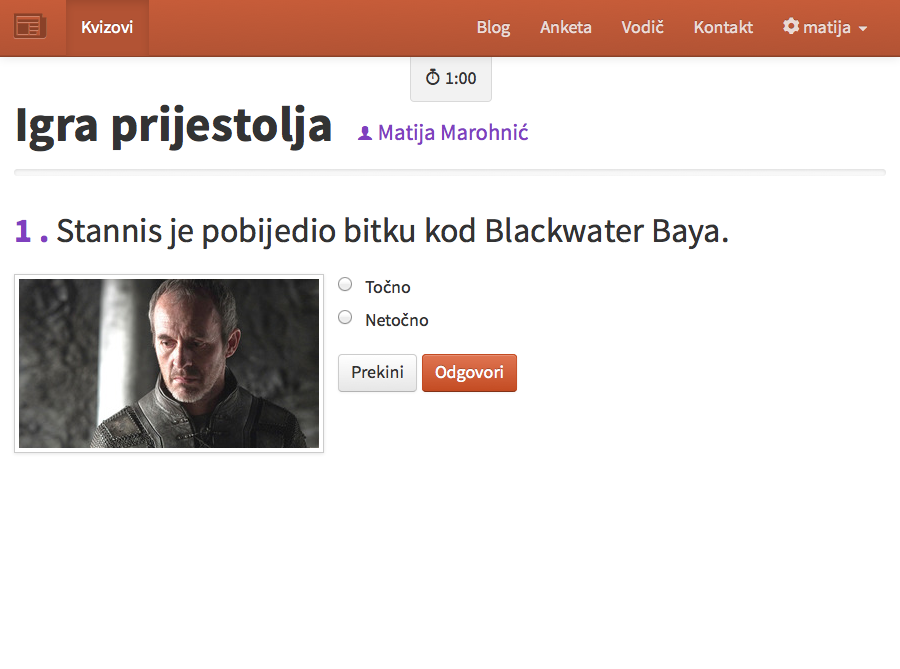
\includegraphics[width=\textwidth, clip=true, trim=0 7cm 0 0, fbox]{student/boolean_question}
  \caption{Pitanje vrste \emph{točno/netočno}}
  \label{fig:boolean}
\end{figure}

\subsection{Ponuđeni odgovori}

\emph{Ponuđeni odgovori} (slika \ref{fig:choice}) je vrsta pitanja gdje se
postavlja pitanje na koje treba odgovoriti \textbf{jednim} od ponuđenih
odgovora. Ova vrsta pitanja je teža od \emph{točno/netočno} jer se vjerojatnost
da korisnik točno odgovori smanjuje s brojem ponuđenih odgovora.

Premda je postojala mogućnost da se ponudi više točnih odgovora, to bi ipak
uvelike otežalo ovu vrstu pitanja pa je odlučeno da će se odgoditi
implementacija te značajke za jednu od budućih verzija aplikacije.

\begin{figure}[H]
  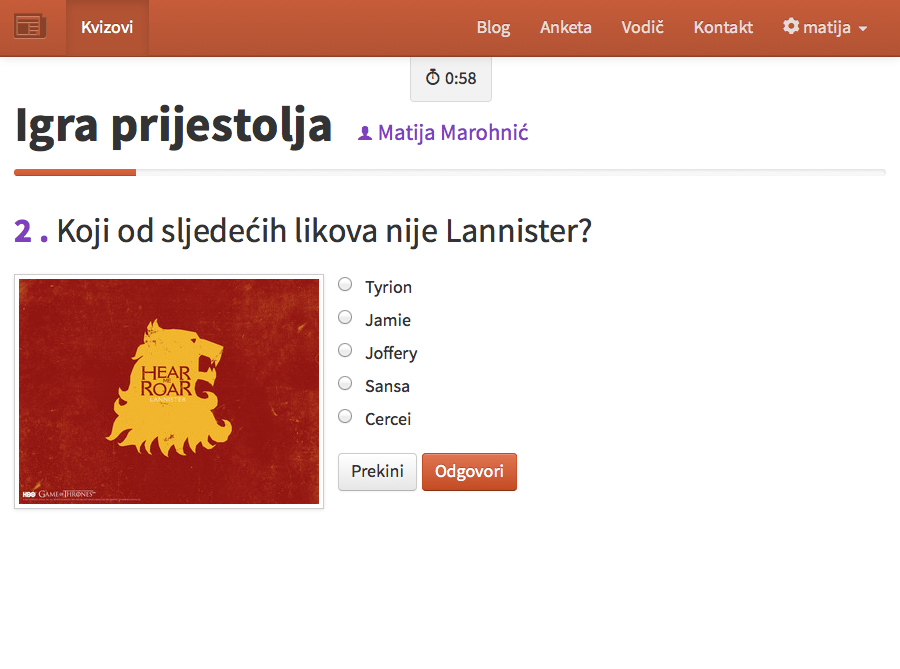
\includegraphics[width=\textwidth, clip=true, trim=0 5cm 0 0, fbox]{student/choice_question}
  \caption{Pitanje vrste \emph{ponuđeni odgovori}}
  \label{fig:choice}
\end{figure}

\subsection{Asocijacija}

\emph{Asocijacija} (slika \ref{fig:association}) je vrsta pitanja gdje korisnik
pridružuje pojmove iz jednog s pojmovima iz drugog stupca. Ovo pitanje je teže
od \emph{ponuđenih odgovora} jer se broj mogućih kombinacija eksponencijalno
povećava s brojem parova pojmova.

\begin{figure}[H]
  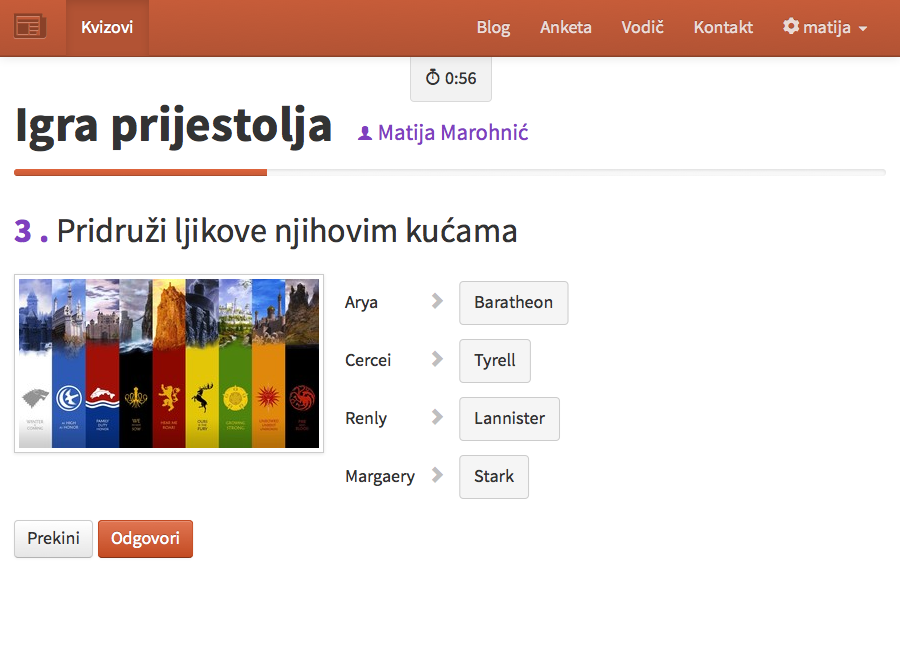
\includegraphics[width=\textwidth, clip=true, trim=0 3cm 0 0, fbox]{student/association_question}
  \caption{Pitanje vrste \emph{asocijacija}}
  \label{fig:association}
\end{figure}

Ova vrsta pitanja bila je tehnički složenija za oblikovanje jer postoji mnogo
različitih pristupa. Odlučili smo se za pristup gdje se pojmovi ``primaju'' s
mišem i ``ispuštaju'' na drugi pojam nakon čega ta 2 pojma zamjenjuju mjesta.
Na taj način korisnik može preslagivati pojmove dok ne dobije željenu
kombinaciju.

\subsection{Upiši točan odgovor}

\emph{Upiši točan odgovor} (slika \ref{fig:text}) je vrsta pitanja gdje se
postavlja pitanje, a korisnik treba upisati točan odgovor u za to predviđeno
tekstno polje. Ova vrsta pitanja je najteža zato što je vrlo lako pogriješiti
-- korisnik mora upisati odgovor točno onako kako ga je administrator napisao.

\begin{figure}[H]
  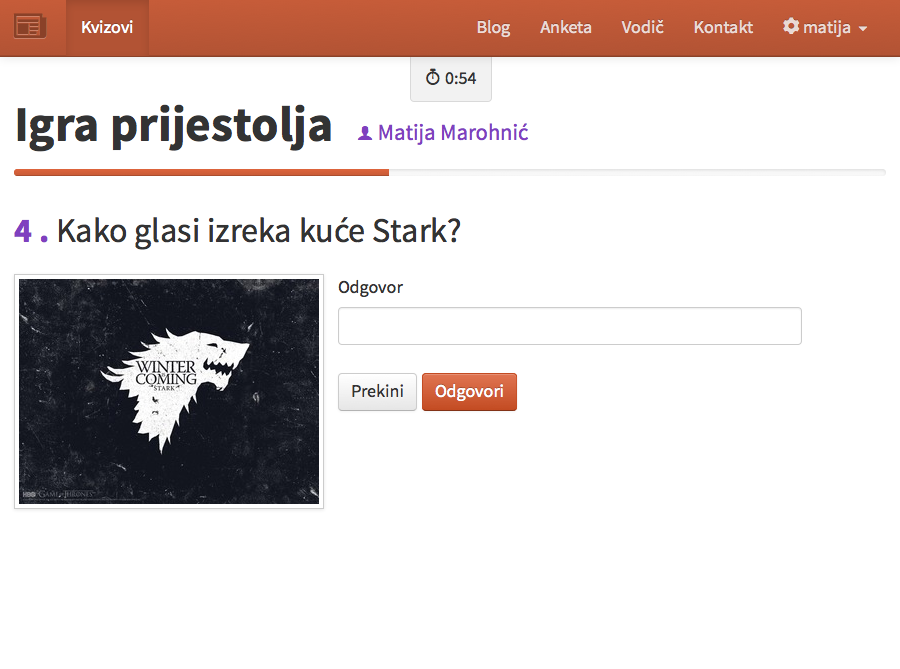
\includegraphics[width=\textwidth, clip=true, trim=0 5cm 0 0, fbox]{student/text_question}
  \caption{Pitanje vrste \emph{upiši točan odgovor}}
  \label{fig:text}
\end{figure}

Kako bismo učinili ovu vrstu pitanja malo lakšom, dizajnirali smo je tako da
nije bitno piše li korisnik malim ili velikim slovima; ako se slova podudaraju
s točnim odgovorom, ponuđeni se odgovor smatra točnim.

\section{Iz perspektive korisnika}

\subsection{Nastavnici}

\emph{Škola} je uloga koja predstavlja profesora i ona je administrator kvizova.

Nakon odabira te uloge korisnik se može prijaviti ili registrirati ako još nema
korisnički račun. Registracija se sastoji od ispunjavanja jednostavnog
formulara pomoću kojega prikupljamo informacije o korisnicima koje možemo
iskoristiti kako bismo poboljšali njihovo iskustvo i kako bismo mogli raditi
istraživanja. Polje u formularu za registraciju na koje ćemo se osvrnuti je
\emph{Tajni ključ}, koji je potreban za registraciju učenicima te škole.

Nakon prijave nastavnicima se otvara stranica s popisom kvizova koje su
kreirali (vidi sliku \ref{fig:school/quizzes}),

\begin{figure}[H]
  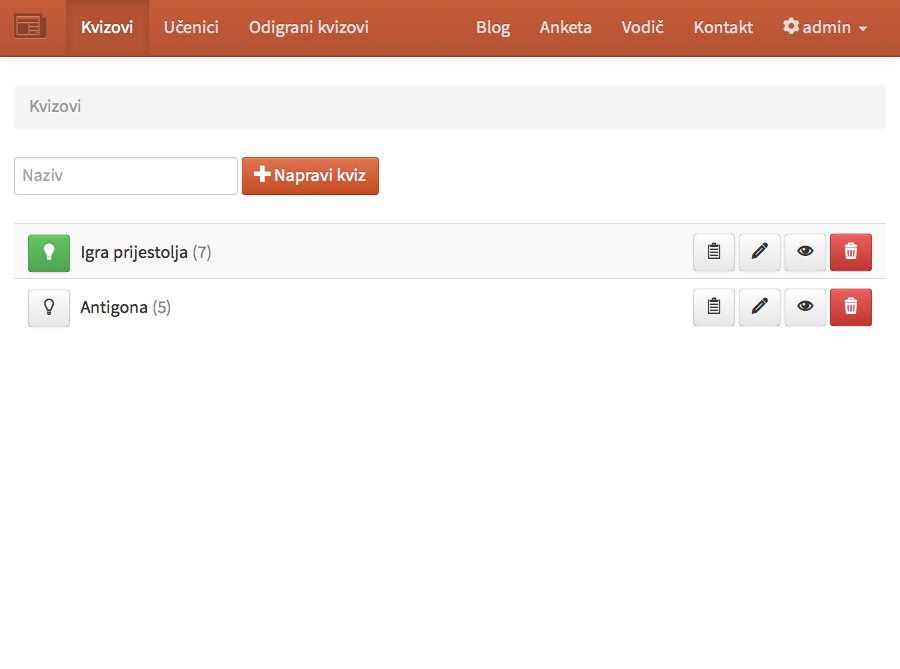
\includegraphics[width=\textwidth, clip=true, trim=0 10cm 0 0, fbox]{school/quizzes}
  \caption{Škole -- popis kvizova}
  \label{fig:school/quizzes}
\end{figure}

gdje mogu izmjenjivati postojeće kvizove i sastavljati nove. Nakon što je
profesor dovršio izradu kviza, može ga učiniti aktivnim, odnosno vidljivim
učenicima. Izmjenjivanje kvizova podijeljeno je na izmjenu metapodataka kviza i
na izmjenu pitanja kviza. Ovdje napominjemo da ćemo, zbog zaštite privatnosti
naših korisnika, u radu prikazivati podatke kviza koji smo sami napravili (Igra
prijestolja), a našim imenima ćemo zamijeniti stvarna imena korisnika koji su
sudjelovali u istraživanju.

Uz svako se pitanje može pridružiti pomoć (slikom ili tekstom) koja će se
prikazati učenicima dok rješavaju pitanje.

Škole mogu pregledavati informacije o odigranim kvizovima: kada su odigrani,
tko ih je igrao, koji su ukupni rezultati itd. (vidi sliku \ref{played_quizzes}).

\begin{figure}[H]
  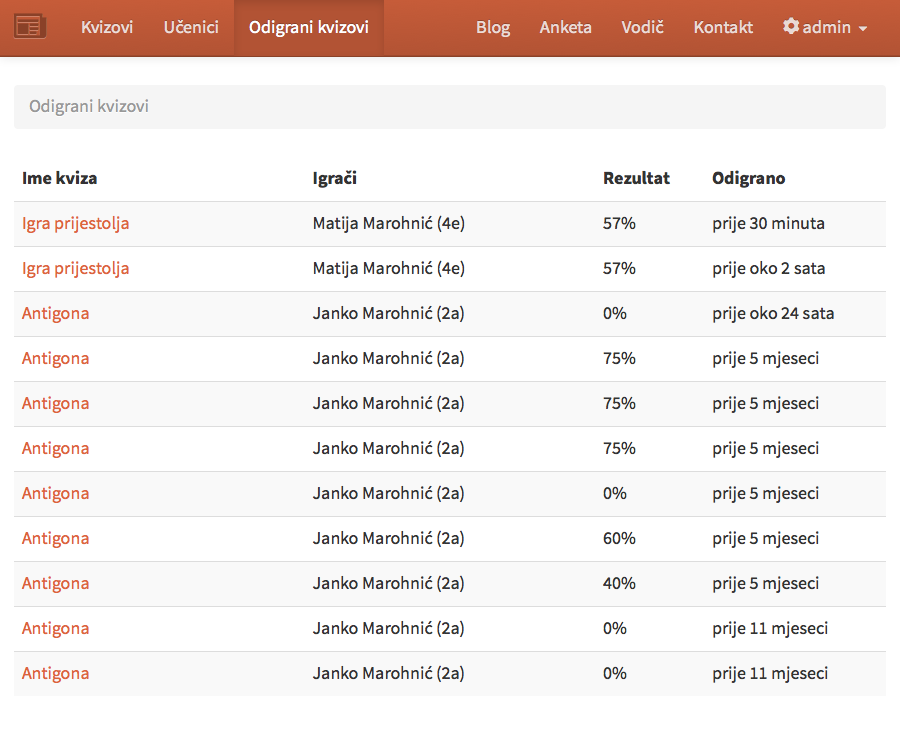
\includegraphics[width=\textwidth, clip=true, trim=0 10cm 0 0, fbox]{school/played_quizzes}
  \caption{Škole -- sažeti podaci o odigranim kvizovima}
  \label{played_quizzes}
\end{figure}

Ali isto tako može se pristupiti svakom odigranom kvizu i detaljno pregledati
svi odgovori (vidi sliku \ref{played_quiz}).

\begin{figure}[H]
  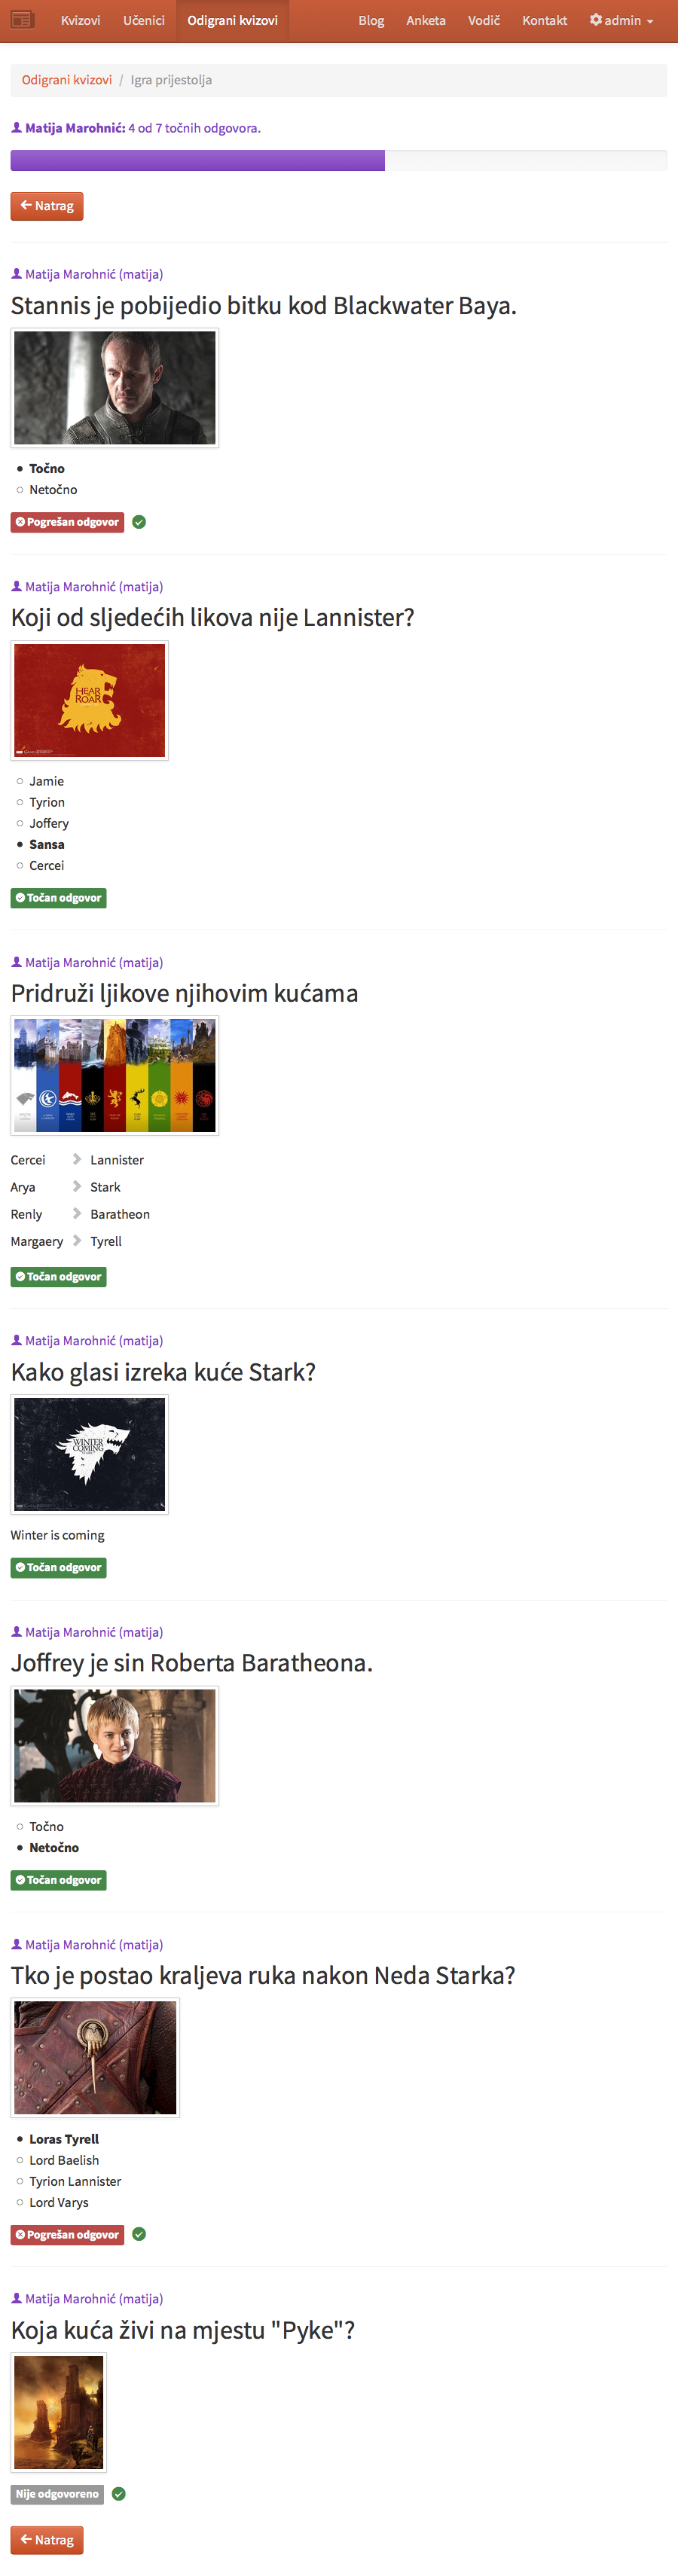
\includegraphics[width=\textwidth, clip=true, trim=0 80cm 0 0, fbox]{school/played_quiz}
  \caption{Detaljan pregled rezultata kviza}
  \label{played_quiz}
\end{figure}

Mogu se pregledavati i profili učenika, koliko su kvizova odigrali, koji su to
kvizovi i sl. (vidi sliku \ref{students}).

\begin{figure}[H]
  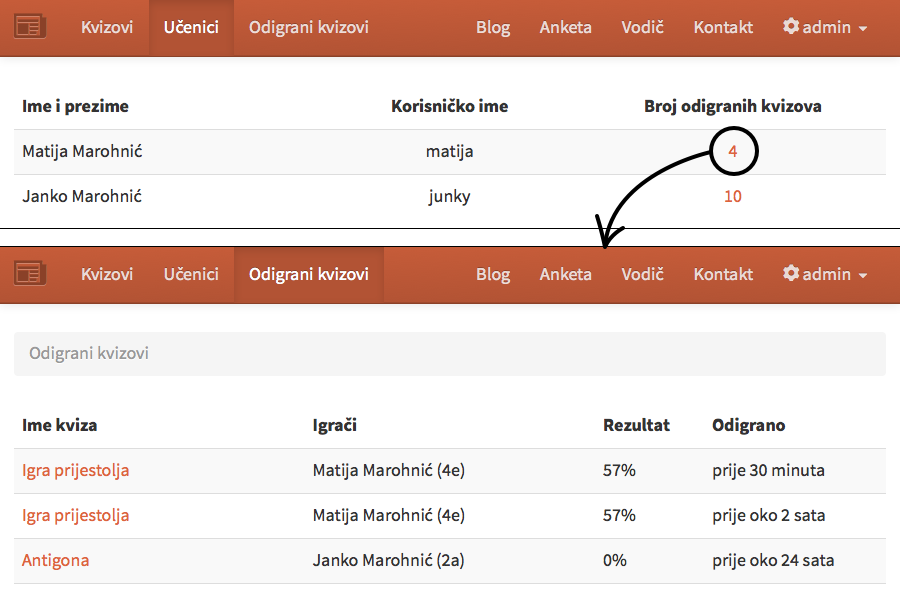
\includegraphics[width=\textwidth, clip=true, trim=0 0 0 0, fbox]{school/students_details}
  \caption{Škole -- pojedinačni pregled odigranih kvizova po svakom učeniku}
  \label{students}
\end{figure}

\subsection{Učenici}

\emph{Učenik} je uloga koja rješava kvizove koje je napravila njihova škola.
Kao i kod škole, učenik se može prijaviti ili registrirati ako već nema
korisnički račun. Pri registraciji učenik treba napisati tajni ključ koji mu je
njegova škola dala, u protivnom se ne može registrirati. Na taj način
sprječavamo da se bilo tko registrira kao učenik.

Nakon prijave ili registracije, korisnika dočeka lista kvizova koji su dostupni
za rješavanje. Kviz je moguće igrati samostalno, ali i u paru (vidi sliku
\ref{student/quizzes}). U drugom slučaju drugi igrač također mora biti
prijavljen u sustav.

\begin{figure}[H]
  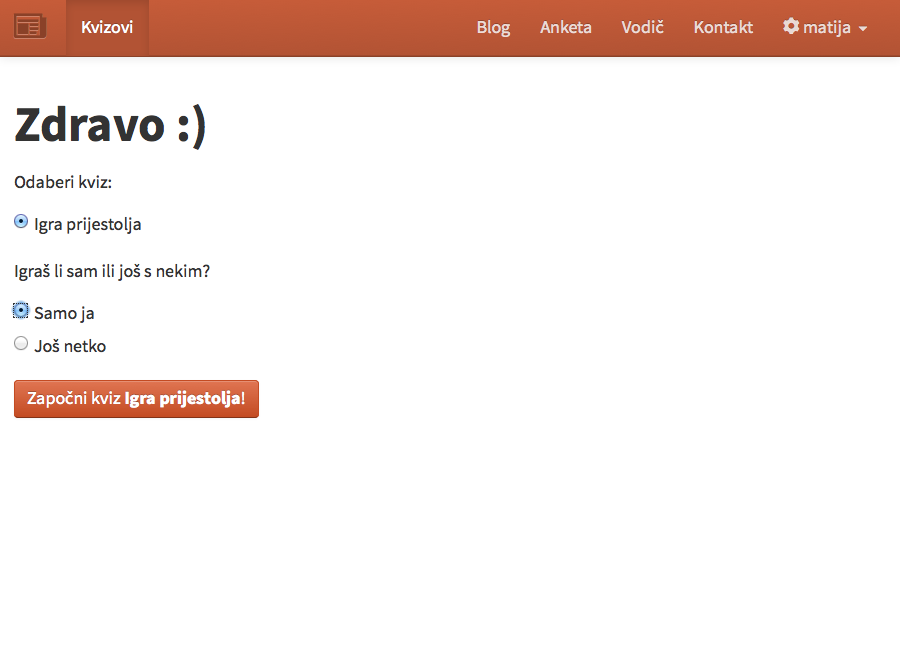
\includegraphics[width=\textwidth, clip=true, trim=0 8.5cm 0 0, fbox]{student/quizzes}
  \caption{Učenici -- popis kvizova}
  \label{student/quizzes}
\end{figure}

Nakon što učenik započne kviz, prikazuje mu se jedno po jedno pitanje na koje
treba odgovoriti. Kako bi igra bila što pravilnija, pitanja su obično vremenski
ograničena, tako da učenik ne može koristiti druge izvore informacija.
Preostalo vrijeme ispisano je iznad imena korisnika (vidi sliku
\ref{question}).

\begin{figure}[H]
  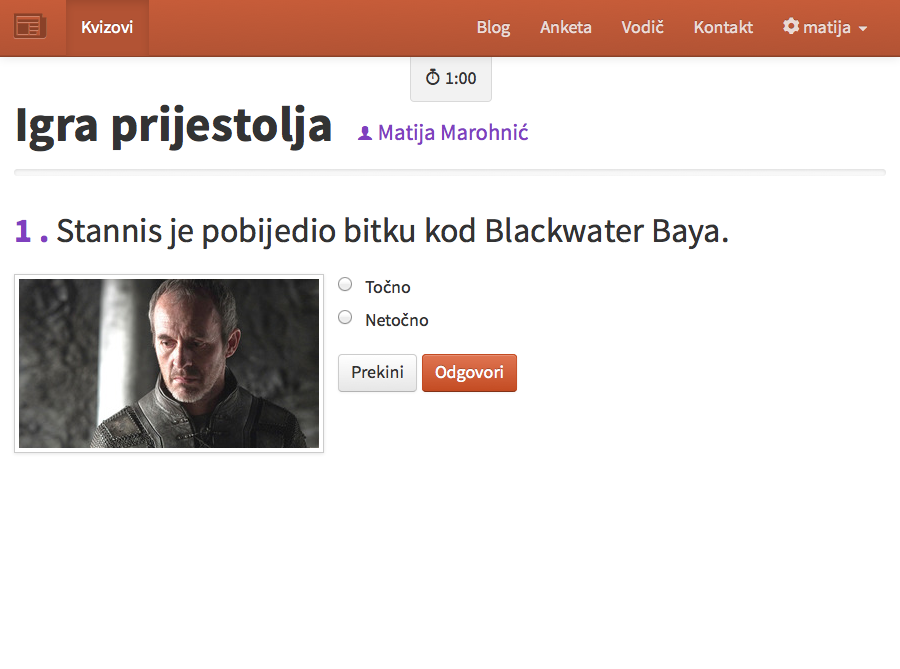
\includegraphics[width=\textwidth, clip=true, trim=0 7cm 0 0, fbox]{student/boolean_question}
  \caption{Učenici -- odgovaranje na pitanje}
  \label{question}
\end{figure}

Nakon što učenik potvrdi odgovor pritoskom na gumb \emph{Odgovori}, prikaže mu
se i poruka o točnosti odgovora s gumbima za prelazak na sljedeće pitanje (vidi
sliku \ref{fig:feedback}).

\begin{figure}[H]
  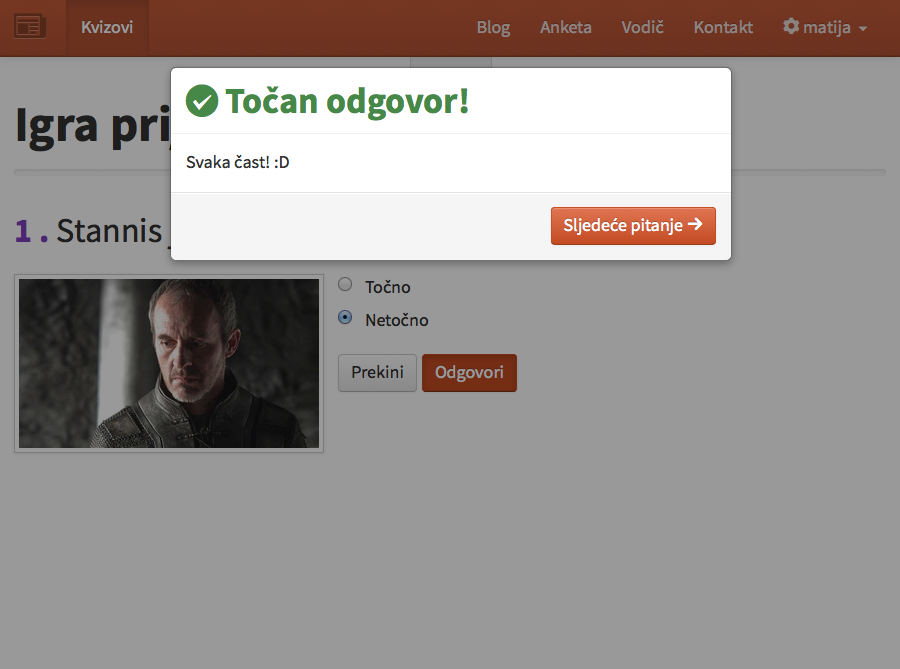
\includegraphics[width=\textwidth, clip=true, trim=0 7cm 0 0, fbox]{student/boolean_question_correct}
  \caption{Učenici -- povratna informacija nakon točnog odgovora na pitanje}
  \label{fig:feedback}
\end{figure}

Nakon što učenik odgovori na sva pitanja, ispisuju se rezultati i učenik dobiva
određenu ``titulu'' s obzirom na njegov rezultat:

\begin{center}
  \begin{tabular}{lll}
    0\%-29\%   & -- & \textbf{Znalac-šegrt}  \\
    30\%-49\%  & -- & \textbf{Znalac-malac}  \\
    50\%-74\%  & -- & \textbf{Znalac}        \\
    75\%-84\%  & -- & \textbf{Ekspert}       \\
    85\%-94\%  & -- & \textbf{Super ekspert} \\
    95\%-100\% & -- & \textbf{Čarobnjak}     \\
  \end{tabular}
\end{center}

Titule su osmišljene zato da se učenika uvijek pohvaljuje čak i ako je imao loš
rezultat, tako da se učenik dobro osjeća i da ga se potiče da igra i dalje.

Osim zbog interaktivnosti, ovakav način podučavanja dobro funkcionira zato što
možemo na licu mjesta ispravljati greške i ažurirati aplikaciju prema povratnim
informacijama dok je učenici i profesori koriste. I profesori mogu relativno
brzo i jednostavno unositi izmjene u testove ili pak ispravljati uočene greške.
Sve njihove promjene odmah stupaju na snagu i dostupne su učenicima.

\chapter{Rezultati}
\label{chap:results}

Mogli bismo reći da smo aplikaciju izrađivali u 3 faze.

U 1. fazi smo radili aplikaciju, od 9.7.2012. do 22.8.2012.

U 2. fazi smo prvu verziju dali na korištenje u 5 testnih škola u periodu
22.8.2012 do 16.5.2013. U toj je fazi sudjelovalo 5 profesora i 254 učenika. Na
kraju 2. faze proveli smo i anketiranje čije rezultate ćemo prikazati
detaljnije u ovom poglavlju.

u 3. fazi, u projekt su se uključile i ostale škole pa je broj nastavnika
porastao na 20 a broj učenika na 401. Moramo napomenuti da škole koje su se
priključile projektu u ovoj 3. fazi nisu bile iz kontroliranog uzorka škola već
su samoinicijativno odlučile koristiti program. U ovoj fazi nismo provodili
dodatno anektiranje korisnika već smo se više posvetili dorađivanju same
aplikacije.

\section{Škole}

Anketa je pokazala da je većina profesora primijetila napredak u poznavanju
gradiva kod svojih učenika, kao i veću zainteresiranost za gradivo (vidi slike
\ref{fig:school/advance}, \ref{fig:school/comparison} i \ref{fig:school/help}).

\begin{figure}[H]
  \centering
  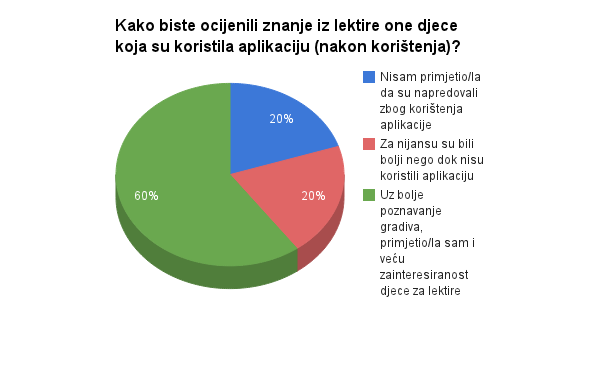
\includegraphics[scale=0.7]{school/advance}
  \caption{Napredak učenika}
  \label{fig:school/advance}
\end{figure}

\begin{figure}[H]
  \centering
  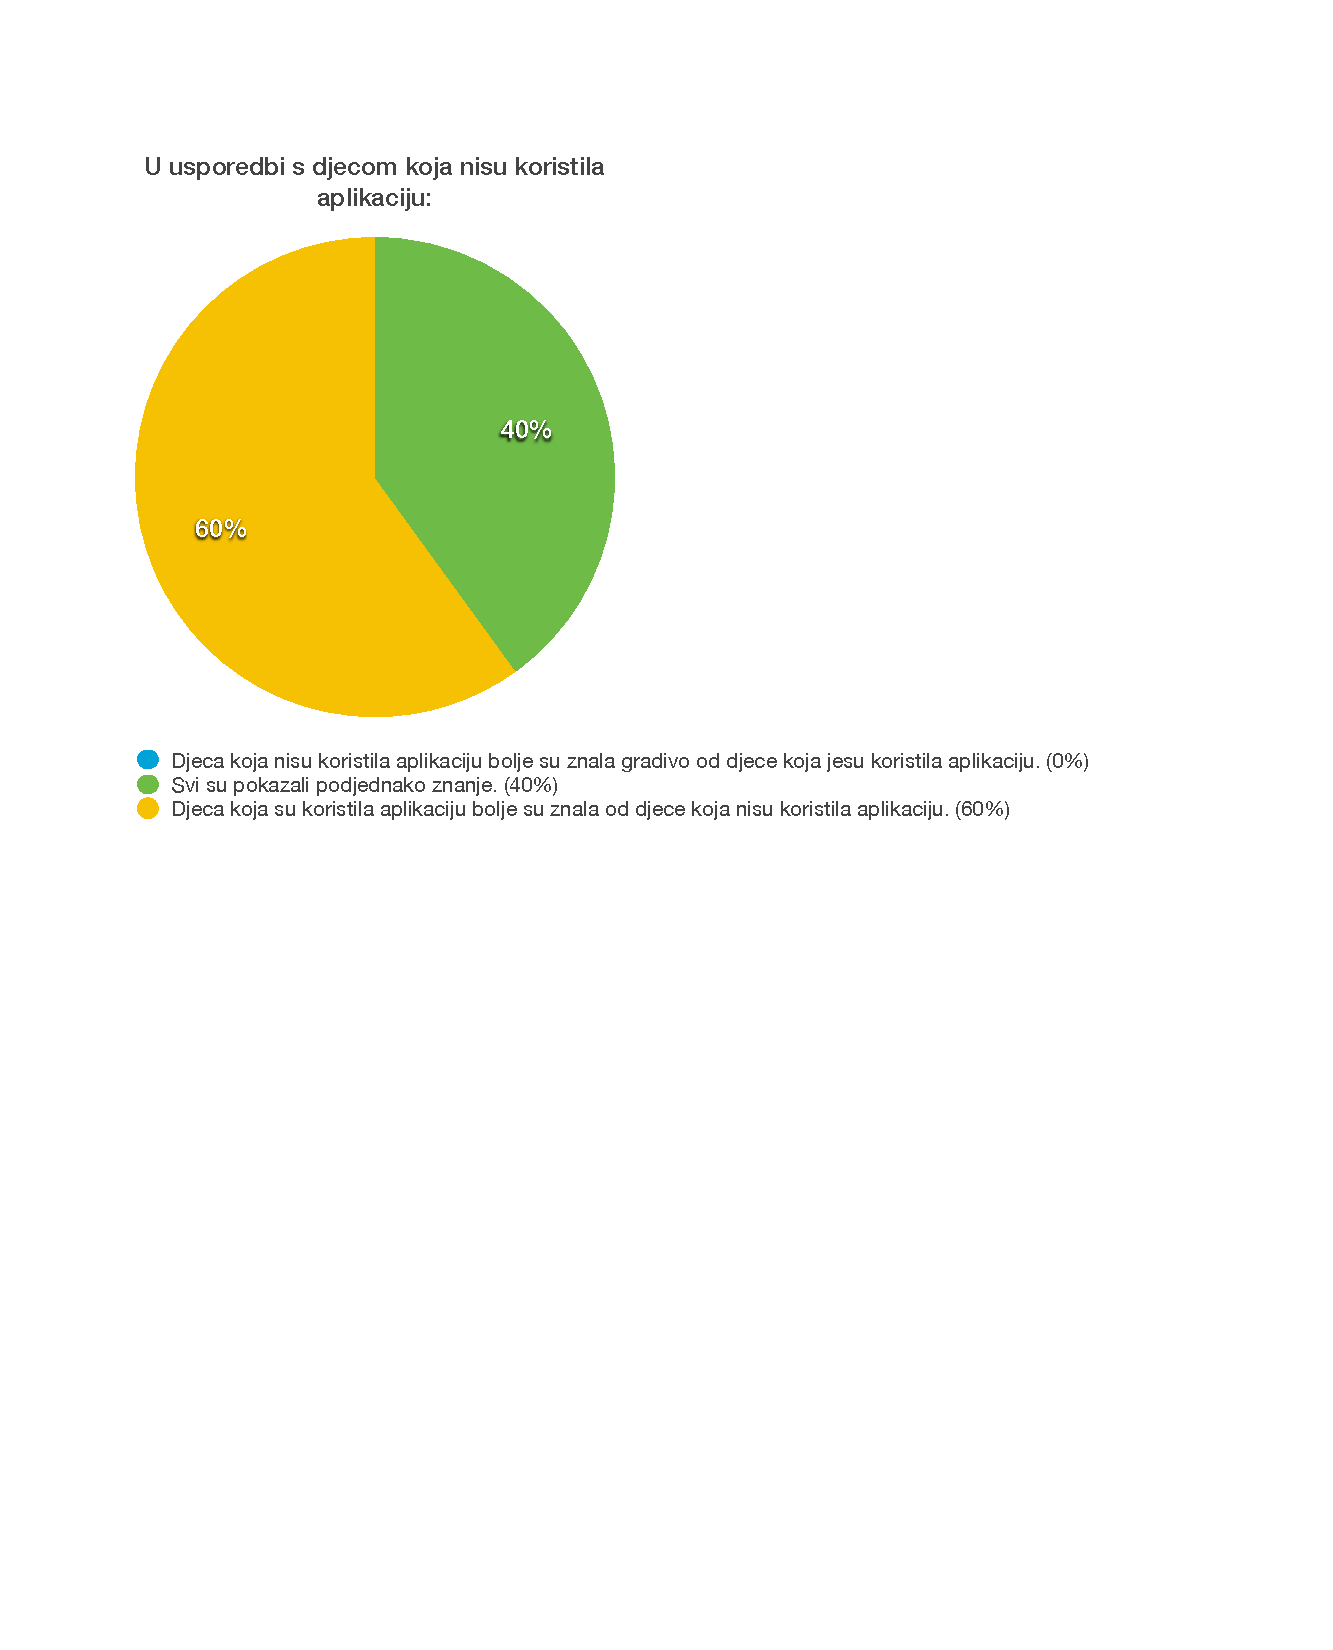
\includegraphics[scale=0.7]{school/comparison}
  \caption{Usporedba učenika koji su koristili aplikaciju s onima koji nisu}
  \label{fig:school/comparison}
\end{figure}

\begin{figure}[H]
  \centering
  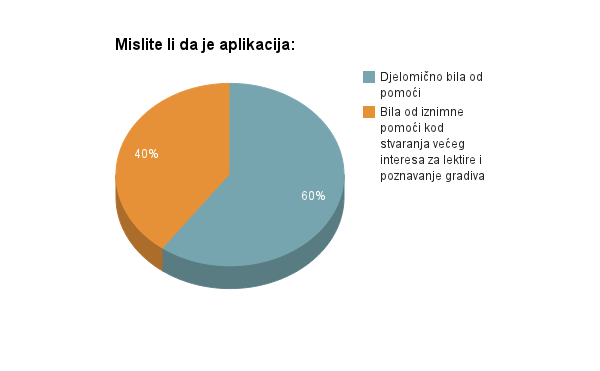
\includegraphics[scale=0.7]{school/help}
  \caption{Poticanje interesa učenika za gradivo}
  \label{fig:school/help}
\end{figure}

\section{Učenici}

Kod učenika je anketa pokazala da učenici
smatraju ovakav način učenja učinkovitim (vidi slike
\ref{fig:student/interesting}, \ref{fig:student/effective} i
\ref{fig:student/help}).

S druge strane, anketa je pokazala da je tek pola učenika osjetilo napredak u
ocjeni (vidi sliku \ref{fig:student/grades}).

\begin{figure}[H]
  \centering
  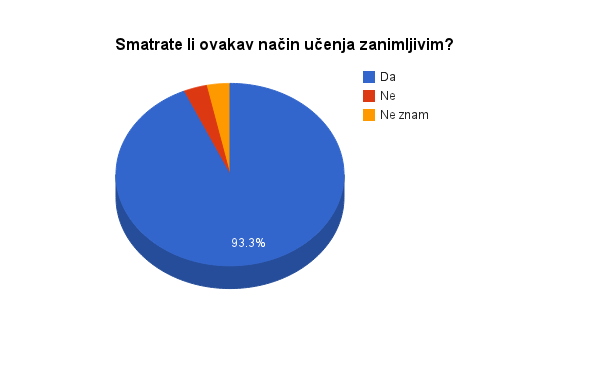
\includegraphics[scale=0.7]{student/interesting}
  \caption{Zanimljivost učenicima}
  \label{fig:student/interesting}
\end{figure}

\begin{figure}[H]
  \centering
  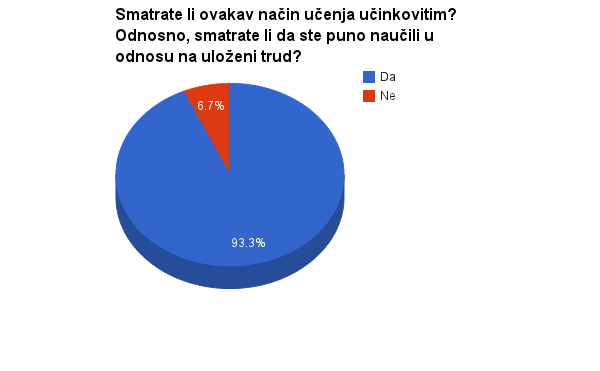
\includegraphics[scale=0.7]{student/effective}
  \caption{Učinkovitost učenicima}
  \label{fig:student/effective}
\end{figure}

\begin{figure}[H]
  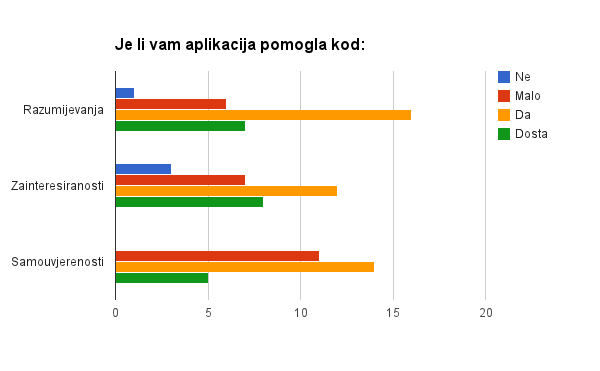
\includegraphics[scale=0.7]{student/help}
  \caption{Pomoć učenicima pri razumijevanju, zainteresiranosti i samouvjerenosti}
  \label{fig:student/help}
\end{figure}

\begin{figure}[H]
  \centering
  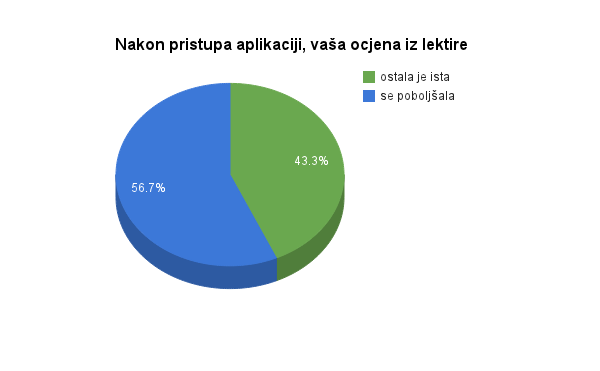
\includegraphics[scale=0.7]{student/grades}
  \caption{Promjena ocjene kod učenika}
  \label{fig:student/grades}
\end{figure}

\chapter{Zaključak}

Prema rezultatima koje smo dobili i detaljno prikazali u poglavlju 4, vjerujemo
da smo opravdali ciljeve postavljene u poglavlju 2. Uspjeli smo i pomoći
učenicima da bolje savladaju gradivo (čak njih 50\% ima veću ocjenu) a i
profesorima smo podučavanje učinili zanimljivijim (njih 80\% bi aplikaciju
preporučilo ne samo svojim kolegama prof. hrvat. jezika već i ostalim
nastavnicama).

I dalje se nastoji pojednostavniti sučelje aplikacije tako da vodič za
aplikaciju više neće biti potreban te da bude jasno samo po sebi kako postići
određeni cilj. Iako aplikaciju mogu koristiti korisnici koji nisu najvještiji u
korištenju web aplikacija, vjerujemo da svi korisnici više vole učiti iz prakse
a ne čitati upute, i da aplikaciju možemo učinit dovoljno jednostavnom da je
pristupačna za svaki uzrast i stupanj informatičke obrazovanosti.

Aplikacija \emph{Kvizovi} je prvotno nastala kao pomoćno sredstvo za učenje
lektira, ali s obzirom na pozitivan utjecaj na učenike i profesore i rezultate
iz anketa više ne vidimo razlog zašto se aplikacija ne bi koristila i za ostale
školske predmete kao što su zemljopis, biologija, kemija itd.

\chapter{Zahvale}

Zahvaljujemo našoj mentorici, doc. dr. sc. Kristini Kocijan na ideji aplikacije
\emph{Kvizovi}, strukturiranju ovoga rada, na prikupljanju uzorka škola koje su
bile voljne koristiti našu aplikaciju i velikom strpljenju tijekom dviju godina
rada na projektu. Također zahvaljujemo kolegici Marti Mihaljević na jezičnim
savjetima. Nadalje, htjeli bismo zahvaliti profesorima i učenicima iz ispitanog
uzorka na sudjelovanju u ovom istraživanju i na slanju prijedloga i prijavu
grešaka što nam je puno pomoglo u razvijanju aplikacije.

Poredane prema broju aktivnih kvizova, škole koje su sudjelovale u istraživanju
su: Prva gimnazija, Osnovna škola Bogumila Tonija, Osnovna škola Stjepana
Radića, Srednja škola Metković, Osnovna škola Poreč, Osnovna škola Stubičke
Toplice, Gimnazija Sesvete, Poljoprivredna škola, Srednja škola ``Ivan
Seljanec'' Križevci, Gimnazija fra Dominika Mandica, Medicinska škola Varaždin,
Srednja škola Čakovec, Tehnička škola Šibenik, Privatna srednja ekonomska škola
INOVA, Škola za umjetnost, dizajn, grafiku i odjeću Zabok, Gimnazija i
strukovna škola Jurja Dobrile i Nadbiskupska klasična gimnazija.

\renewcommand{\listoffigures}{\begingroup
\tocchapter
\tocfile{\listfigurename}{lof}
\endgroup}

\listoffigures

\renewcommand{\bibname}{Popis literature}

\begin{thebibliography}{99}

  \raggedright

  \bibitem{perisic13} Perišić, K. Kako poboljšati koncentraciju djeteta? //
    Klokanica.hr (2013.) URL:
    \url{http://www.klokanica.hr/skolarci/skola/kako-poboljsati-koncentraciju-djeteta-168}.
    (23.4.2014.).

  \bibitem{clark11} Clark, D. Visual, Auditory, and Kinesthetic Learning Styles
    (VAK). // The Performance Juxtaposition (2011.) URL:
    \url{http://www.nwlink.com/~donclark/hrd/styles/vakt.html}. (23.4.2014.).

  \bibitem{htmlncss} HTML \& CSS - W3C. // W3C (2014.) URL:
    \url{http://www.w3.org/standards/webdesign/htmlcss}. (30.4.2014.).

  \bibitem{diveintohtml5} Pilgrim, M. Five Things You Should Know About HTML5 -
    Dive Into HTML5 // Dive Into HTML5 (2012.) URL:
    \url{http://mislav.uniqpath.com/diveintohtml5/introduction.html}.
    (30.4.2014.).

  \bibitem{js} JavaScript Web APIs - W3C. // W3C (2014.)
    \url{http://www.w3.org/standards/webdesign/script}. (30.4.2014.).

  \bibitem{effectivejs} Herman, D. Effective JavaScript : 68 Specific Ways to
    Harness the Power of JavaScript. // Effective Software Development Series.
    Addison-Wesley Professional (2012.)

  \bibitem{mdnjs} Mozilla, Inc. JavaScript Overview - JavaScript | MDN //
    Mozilla Developer Network (2014.) URL:
    \url{https://developer.mozilla.org/en-US/docs/Web/JavaScript/Guide/JavaScript_Overview}.
    (30.4.2014.).

  \bibitem{git} GitHub, Inc. Git - Documentation. (2014.) URL:
    \url{http://git-scm.com/documentation}. (29.4.2014.).

  \bibitem{gauges} GitHub, Inc. Documentation - Gauges // Gauges (2014.) URL:
    \url{http://get.gaug.es/documentation/}. (29.4.2014.).

  \bibitem{github} GitHub, Inc. GitHub · Build Software Better, Together. //
    GitHub (2014.) URL: \url{https://github.com/}. (29.4.2014.).

  \bibitem{mit} GitHub, Inc. MIT License - ChooseALicense.com. //
    ChooseALicense.com (2014.) URL:
    \url{http://choosealicense.com/licenses/mit/}. (29.4.2014.).

  \bibitem{ruby} Documentation. // Ruby (2014.) URL:
    \url{https://www.ruby-lang.org/en/documentation/}. (29.4.2014.).

  \bibitem{postgresql} PostgreSQL: Documentation: 9.3:  What is PostgreSQL? //
    PostgreSQL (2014.) URL:
    \url{http://www.postgresql.org/docs/9.3/interactive/intro-whatis.html}.
    (29.4.2014.).

  \bibitem{heroku} Heroku | Cloud Application Platform. // Heroku (2014.) URL:
    \url{https://www.heroku.com/}. (29.4.2014.).

  \bibitem{krug05} Krug, S. Don’t Make Me Think! : A Common Sense Approach to
    Web Usability. 2nd Edition. / New York: New Riders, 2005.

  \bibitem{kvizovinet} Kvizovi.net :: Znanje je sexy ;-). // Kvizovi.net (2014.)
    URL: \url{http://kvizovi.net/}. (28.4.2014.).

  \bibitem{kvizoteka} kvizovi | kvizovi znanja | kviz igre | nagradni kvizovi |
    KVIZOTEKA. // Kvizoteka (2014.) URL: \url{http://www.kvizoteka.net/}.
    (28.4.2014.).

  \bibitem{ucionica} Wargog. Ucionica on the App Store on iTunes. // iTunes
    (2014.) URL:
    \url{https://itunes.apple.com/hr/app/ucionica/id566902215?mt=8}.
    (28.4.2014.).

  \bibitem{quizup} Plain Vanilla Corp. QuizUp™ on the App Store on iTunes. //
    iTunes (2014.) URL:
    \url{https://itunes.apple.com/hr/app/quizup/id718421443?mt=8}. (28.4.2014.).

\end{thebibliography}

\chapter{Sažetak}

Upotreba web aplikacije za kvizove u nastavi osnovnih i srednjih škola

Matija Marohnić, Janko Marohnić

Zbog sveprisutnosti tehnologije učenici u školama ne osjećaju više istu
učinkovitost tradicionalnih načina učenja. Učenici bolje uče i više se zanimaju
za gradivo kroz medije koji su interaktivniji.

Izradili smo web aplikaciju \textit{Kvizovi} koja pruža mogućnost profesorima u
školama da svojim učenicima sastavljaju kvizove vezane uz gradivo koje
podučavaju. Učenici mogu igrati kvizove svojih škola, a profesori mogu
promatrati rezultate tih odigranih kvizova, promatrati kvalitetu pitanja i
odgovora itd. Hipoteza istraživanja je da će učenicima ovakav način učenja biti
zanimljiviji i da će se više zainteresirati za gradivo.

Nakon postavljanja aplikacije na Internet, uz pomoć naše mentorice smo našli
škole i učenike koji su pristali testirati aplikaciju. Nakon nekog vremena smo
anketom ispitali škole i učenike da bismo saznali koliko je aplikacija bila
korisna.

Anketa je pokazala da je učenicima takav način učenja bio učinkovit i
zanimljiv, i da je 50\% njih osjetilo promjenu u ocjeni na bolje. Profesori su
primijetili napredak svojih učenika kao i veću zainteresiranost za gradivo.

\textbf{Ključne riječi}: kvizovi, web aplikacija, interaktivno učenje,
alternativno podučavanje, nove tehnologije u nastavi

\chapter{Summary}

Usage of a web application for quizzes in class of primary and high schools

Matija Marohnić, Janko Marohnić

Because of omnipresence of technology, students in schools don't feel the
traditional ways of learning is having the same effectiveness. Students learn
better and are more interested in the school matter through more interactive
medias.

We developed a web application \textit{Quizzes}, which gives the ability for
teachers in schools to make quizzes for their students connected with the
matter they're teaching. Students can play quizzes made by their school, and
teachers can monitor the results of the played quizzes, the quality of
questions and answers etc. Hypothesis of the research is that for students this
way of learning will be more interesting and will make them more interested in
the matter in general.

After making the application available online, with the help of our mentor we
managed to find schools which were willing to test the application. After a
certain period of time we gave them surveys with the goal of finding out how
useful was the application to them.

The surveys have shown that students find this way of learning more effective
and interesting, and 50\% of them felt that their grade improved. The teachers
noticed improvement of their students, as well as a general raise in interest
of students for the matter.

\textbf{Keywords}: quizzes, web application, interactive learning, alternative
teaching, new technologies in class

\end{document}
